% Checklist before submitting:
% - [X] Set toggles below to all zeros
% - [X] Grep for "TODO"
% - [X] Put \balance command in the right place to balance columns on last page
% - [ ] Add a label in Overleaf to mark the submitted version
% - [ ] Sync to github.com/dreeves/oddable

%%%%%%%%%%%%%%%%%%%%%%%%%%%%%%%%%%%%%%%%%%%%%%%%%%%%%%%%%%%%%%%%%%%%%%%%%%%%%%%%
%%%%%%%%%%%%%%%%%%%%%%%%%%% SUBMISSION INSTRUCTIONS %%%%%%%%%%%%%%%%%%%%%%%%%%%%
%%%%%%%%%%%%%%%%%%%%%%%%%%%%%%%%%%%%%%%%%%%%%%%%%%%%%%%%%%%%%%%%%%%%%%%%%%%%%%%%

%%% LaTeX Template for AAMAS-2021 (based on sample-sigconf.tex)
%%% Prepared by Natasha Alechina and Ulle Endriss (version 2020-08-06)

%%% Submissions are limited to 4 pages in length in the AAMAS-2021 format, with 
%%% any additional pages containing only bibliographic references.

%%% Due: 2020-12-08 (maybe as late as 7am eastern the morning of Dec 9)

%%%%%%%%%%%%%%%%%%%%%%%%%%%%%%%%%%%%%%%%%%%%%%%%%%%%%%%%%%%%%%%%%%%%%%%%%%%%%%%%
%%%%%%%%%%%%%%%%%%%%%%%%% TOGGLES, CONSTANTS, SETTINGS %%%%%%%%%%%%%%%%%%%%%%%%%
%%%%%%%%%%%%%%%%%%%%%%%%%%%%%%%%%%%%%%%%%%%%%%%%%%%%%%%%%%%%%%%%%%%%%%%%%%%%%%%%

\newcount\Onymous % whether to show our names (opposite of anonymous)
\newcount\Chatty  % whether to show our notes-to-selves in the pdf
\newcount\Stampy  % whether to show a timestamp in the pdf
\newcount\Heady   % whether to show headers on each page
\Onymous = 0 % 0 for submission; 1 for camera-ready
\Chatty  = 0 % 0 for submission & final copy; 1 for draft
\Stampy  = 0 % 0 for submission & final copy; 1 for draft
\Heady   = 0 % 0 for submission & final copy; 1 for draft

%%%%%%%%%%%%%%%%%%%%%%%%%%%%%%%%%%%%%%%%%%%%%%%%%%%%%%%%%%%%%%%%%%%%%%%%%%%%%%%%
%%%%%%%%%%%%%%%%%%%%%%%%% DOCUMENT CLASS AND PACKAGES %%%%%%%%%%%%%%%%%%%%%%%%%%
%%%%%%%%%%%%%%%%%%%%%%%%%%%%%%%%%%%%%%%%%%%%%%%%%%%%%%%%%%%%%%%%%%%%%%%%%%%%%%%%

\ifnum\Onymous=0
  \documentclass[sigconf,anonymous]{aamas}   % this one for submission
\fi\ifnum\Onymous=1 % something weird with aamas.cls preventing an \else here
  \documentclass[sigconf]{aamas}             % this one for final version
\fi

% NB: The AAMAS class file includes many packages already
\usepackage[showseconds=false, showzone=false]{datetime2} % for draft timestamps
% also needs a line like the following in the file latexmkrc:
% $ENV{'TZ'}='America/New_York';

%%%%%%%%%%%%%%%%%%%%%%%%%%%%%%%%%%%%%%%%%%%%%%%%%%%%%%%%%%%%%%%%%%%%%%%%%%%%%%%%
%%%%%%%%%%%%%%%%% AAMAS-2021 COPYRIGHT BLOCK (DO NOT CHANGE!) %%%%%%%%%%%%%%%%%%
%%%%%%%%%%%%%%%%%%%%%%%%%%%%%%%%%%%%%%%%%%%%%%%%%%%%%%%%%%%%%%%%%%%%%%%%%%%%%%%%

\setcopyright{ifaamas}
\acmConference[AAMAS '21]{Proc.\@ of the 20th International Conference on Autonomous Agents and Multiagent Systems (AAMAS 2021)}{May 3--7, 2021}{London, UK}{U.~Endriss, A.~Now\'{e}, F.~Dignum, A.~Lomuscio (eds.)}
\copyrightyear{2021}
\acmYear{2021}
\acmDOI{}
\acmPrice{}
\acmISBN{}

%%%%%%%%%%%%%%%%%%%%%%%%%%%%%%%%%%%%%%%%%%%%%%%%%%%%%%%%%%%%%%%%%%%%%%%%%%%%%%%%
%%%%%%%%%%%%%%%%%%%%%% TITLE, AUTHORS, ABSTRACT, KEYWORDS %%%%%%%%%%%%%%%%%%%%%%
%%%%%%%%%%%%%%%%%%%%%%%%%%%%%%%%%%%%%%%%%%%%%%%%%%%%%%%%%%%%%%%%%%%%%%%%%%%%%%%%

% In anonymous submission mode, this is printed on the first page:
\acmSubmissionID{26} 

\title[
\ifnum\Stampy=1 \tstamp\quad \fi
Confidence in Predictions]{  % short version of title
Towards a Theory of Confidence in Market-Based Predictions} % full title
%Towards a Theory of Confidence in Crowdsourced Probabilistic Predictions}

%%% Provide names, affiliations, and email addresses for all authors.

\author{Rupert Freeman}
\affiliation{
  \institution{University of Virginia}}
\email{freemanr@darden.virginia.edu}

\author{David M. Pennock}
\affiliation{
  \institution{Rutgers University}}
\email{dpennock@dimacs.rutgers.edu}

\author{Daniel M. Reeves}
\affiliation{
  \institution{Beeminder}}
\email{dreeves@beeminder.com}

\author{David Rothschild}
\affiliation{
  \institution{Microsoft Research}}
\email{davidmr@microsoft.com}

\author{Bo Waggoner}
\affiliation{
  \institution{University of Colorado}}
\email{bwag@colorado.edu}

\begin{abstract}
Prediction markets are a way to yield probabilistic predictions about future events, theoretically incorporating all 
%socially 
available information. 
%\dreev{dumb question: what's ``socially available'' mean? i guess just ``available to any participants''. ok, it was clear enough when i actually thought about it! but maybe just ``available'' suffices?}
%In this paper, we ask what, if anything, can be inferred from the market about the information that it has incorporated.
%\dreev{i think the abstract would be clearer/punchier without the previous sentence. i'd even say we should try to cram in the basic idea of god profit in the abstract if we can.}
In this paper, we focus on the \emph{confidence} that we should place in the prediction of a %single
market. 
When should we believe that the market probability meaningfully reflects underlying uncertainty, and when should we not? 
We discuss two notions of confidence. 
The first is based on the expected profit that a trader could make from correcting the market if it were wrong, and the second is based on expected market volatility in the future.
Our paper is a stepping stone to future work in this area, and we conclude by discussing some key challenges.
%We discuss what it means to be confident in a market prediction, propose two notions of confidence that can be inferred from a market, and raise several challenges for future work.
\end{abstract}

\begin{comment}
[experimenting with punchier abstract; i really like abstracts that convey exactly what the paper's contribution is in a few sentences...]
We introduce a metric for a prediction market's confidence: 
dollar-denominated margin of error, defined as a range of probabilities for which an omniscient bettor would make less than a given amount of profit.
We compare it to existing methods like expected volatility and...
\end{comment}


%%% Use this command to specify a few keywords describing your work.
%%% Keywords should be separated by commas. See http://dl.acm.org/ccs.cfm

%\keywords{Prediction Markets, Probability, Forecasting}
%I think we can get away without keywords for the submission

%%%%%%%%%%%%%%%%%%%%%%%%%%%%%%%%%%%%%%%%%%%%%%%%%%%%%%%%%%%%%%%%%%%%%%%%%%%%%%%%
%%%%%%%%%%%%%%%%%%%%%%%%%%%%% COMMANDS AND MACROS %%%%%%%%%%%%%%%%%%%%%%%%%%%%%%
%%%%%%%%%%%%%%%%%%%%%%%%%%%%%%%%%%%%%%%%%%%%%%%%%%%%%%%%%%%%%%%%%%%%%%%%%%%%%%%%

%%%%%%%%%%%%%%%%%%%%%%%%%%%%%%%%%%%%%%%%%%%%%%%%%%%%%%%%%%%%%%%%%%%%%%%%%%%%%%%%

% nothing yet

%%%%%%%%%%%%%%%%%%%%%%%%%%%%%%%%%%%%%%%%%%%%%%%%%%%%%%%%%%%%%%%%%%%%%%%%%%%%%%%%


%\newcommand{\BibTeX}{\rm B\kern-.05em{\sc i\kern-.025em b}\kern-.08em\TeX}

\newcommand{\rupert}[1]{\ifnum\Chatty=1 \textcolor{red}   {Rupert: [#1]} \fi}
\newcommand{\dpenn} [1]{\ifnum\Chatty=1 \textcolor{blue}  {dpenn:  [#1]} \fi}
\newcommand{\dreev} [1]{\ifnum\Chatty=1 \textcolor{purple}{dreev:  [#1]} \fi}
\newcommand{\dmr}   [1]{\ifnum\Chatty=1 \textcolor{orange}{DMR:    [#1]} \fi}
\newcommand{\bo}    [1]{\ifnum\Chatty=1 \textcolor{teal}  {Bo:     [#1]} \fi}

\newcommand{\tstamp}{\textcolor{red}{DRAFT~\DTMnow}}

\hfuzz=2pt % Don't bother to report overfull hboxes if over-edge is < 2pt
\vfuzz=2pt % Same for overfull vboxes (maybe just works for hfuzz?)

%%%%%%%%%%%%%%%%%%%%%%%%%%%%%%%%%%%%%%%%%%%%%%%%%%%%%%%%%%%%%%%%%%%%%%%%%%%%%%%%
%%%%%%%%%%%%%%%%% START DOCUMENT, SET UP HEADERS, DO MAKETITLE %%%%%%%%%%%%%%%%%
%%%%%%%%%%%%%%%%%%%%%%%%%%%%%%%%%%%%%%%%%%%%%%%%%%%%%%%%%%%%%%%%%%%%%%%%%%%%%%%%

\begin{document}

\ifnum\Heady=0
  \ifnum\Stampy=0      % no headers, no "draft" timestamp
    \pagestyle{fancy}  % AAMAS submission version, suppressing all headers
    \fancyhead{}
  \else                % no headers, yes "draft timestamp"
    \fancyhead{}
    \fancypagestyle{firstpage}{
      \lhead{\hfill\tstamp\hfill}}
  \fi
\else
  \ifnum\Stampy=0      % yes headers, no "draft" timestamp
    %nop
  \else                % yes headers, yes "draft" timestamp
    \pagestyle{fancy}
    \fancypagestyle{firstpage}{\lhead{\tstamp}}
  \fi
\fi

%%% The next command prints the information defined in the preamble.

\maketitle
\ifnum\Stampy=1
  \thispagestyle{firstpage}
  \pagenumbering{gobble}
\fi

%%%%%%%%%%%%%%%%%%%%%%%%%%%%%%%%%%%%%%%%%%%%%%%%%%%%%%%%%%%%%%%%%%%%%%%%%%%%%%%%
%%%%%%%%%%%%%%%%%%%%%%%%%%%%%%%% MAIN DOCUMENT %%%%%%%%%%%%%%%%%%%%%%%%%%%%%%%%%
%%%%%%%%%%%%%%%%%%%%%%%%%%%%%%%%%%%%%%%%%%%%%%%%%%%%%%%%%%%%%%%%%%%%%%%%%%%%%%%%

%\vspace{-0.2cm}
\section{Introduction}
\label{sec:intro}

Making probabilistic judgments about the future is fundamental to sound decision making.
An agent may base its predictions on its own direct evidence or on forecasts crowdsourced from others. 
Market-based predictions and other wisdom-of-crowds forecasts, formed by taking an aggregate (e.g., an average, median, or equilibrium) of many individual predictions, tend to be more reliable than domain experts~\cite{tetlock2017expert}. 

All financial markets yield predictions indirectly. 
A \emph{prediction market} is a financial market directly designed to crowdsource predictions. 
Bettors trade securities that eventually realize some value based on the outcome of the event in question. 
The price of the securities at any point in time can be interpreted as a forecast probability that the event occurs.

We have researched the design and use of prediction markets for two decades. 
We have been regular contributors to [redacted for anonymity].
%some of the most high-trafficked mainstream news publications, written op-eds in many others, been interviewed for many articles, and run our own high-profile sites highlighting prediction market forecasts.
%\dreev{almost feels like we're gunning for argument-from-authority there. it would feel less that way if we just matter-of-factly listed those ``high-profile sites'' etc, which of course we can't do, due to anonymity. so maybe we could stick in a ``[redacted for anonymity]'' which might be a stronger argument-from-authority anyway! :) leave it to the reviewers' imaginations who we must be without trying to say explicitly that some of us are a big deal. to be clear, we emphatically are! the above just felt ... i don't know; just an idea, being more strategic about it with ``[redacted for anonymity]'' instead of trying to vague it up.}
The first question many journalists and readers ask is: what is the \textit{margin of error} in a prediction market? What are its confidence bounds?
We don't have good answers. No one does.

A poll has a formula for margin of error.\footnote{In practice, based on the random-sample error, the stated margin of error ignores all of the other error in both data collection and analytics, accounting for roughly half of the total empirically derived error~\cite{shirani2018disentangling}. 
Regardless, polling error is a well-defined concept.}
Although polls are \textit{not} predictions, pundits and consumers regularly compare them, especially during elections, and wonder how to think about the accuracy of, and confidence in, both polls and predictions.
A prediction market has no concept of margin of error, even in theory.
If two markets selling the exact same contract disagree, which should we trust more?
%How can we take conflicting individual and aggregate predictions and use them to generate a single prediction?
How confident can we be in the accuracy of the (aggregated or separate) predictions?
In this paper, we attempt to paint a way forward to answering these questions.

By way of motivation, consider three scenarios predicting the winner of a football match:
\begin{itemize}
\item (Game 1) a normal professional regular-season game 
\item (Game 2) a normal professional regular-season game where, 24 hours before the game, there will be a rapid COVID-19 test to determine the eligibility of the star player 
\item (Game 3) a pick-up game
\end{itemize}
Now imagine that the wisdom of the crowd (via whatever method) gives Team A a 70\% chance of winning 48 hours before the game in all three scenarios. 
Intuitively, that crowd knows that Game 1 is very precisely defined due to years of detailed statistics and precise models.
In Game 2, we will treat it as known that the star player's COVID-19 test is essentially a fair coin flip and that Team A has a 50\% chance of winning without their star and 90\% with them.
That gives a multi-modal future probability~\cite{pearl1987}: %, so to speak: 
0.5*90\% + 0.5*50\% = 70\%.
Finally, the Game 3 estimate is based on scant information; %a crapshoot;
who knows who may show up to play or what may happen?
For all three games, 70\% for Team A is our probability, but that 
70\% 
number is distilling intuitively very different states of uncertainty about the 
%game 
outcomes.

We can model our three games as being faced with a (binary) random number generator that outputs 1 with probability $p$ and 0 with probability $1-p$. 
In Game 1 we are able to observe 10,000 outputs of this random number generator: 
7,000 are 1s and 3,000 are 0s. 
In Game 2 we are able to observe 10,000 outputs of this random number generator under each of the two conditions: we observe 5,000 1s when the test is positive and 9,000 when the test is negative.
%where in a positive test there are 5,000 1s and in a negative test there are 9,000. 
Finally in Game 3 we are only able to observe 10 outputs: 7 1s and 3 0s. 
We assume an %Bayesian
agent with a non-informative prior who concludes 70\% as the probability of 1 in each of the games. %\footnote{Technically the Bayesian has beliefs that differ slightly from 70\%, as given by Laplace's Rule of Succession~\cite{de1840essai}, but this does not affect our underlying question.\rupert{Added this footnote to address the Bayesian/frequentist discussion.}\dpenn{I removed the footnote and the word Bayesian.} \dreev{agree with dpenn; it's a can of worms to get that all technically right and it suffices for our point to just say the conclusion is 70\% in all 3 cases.} 
But what would this agent say when pressed about its confidence, both relative and absolute, for these three games?

%By way of motivation, consider two scenarios. In the first, we are faced with a (binary) random number generator that outputs 1 with probability $p_1$ and 0 with probability $1-p_1$. We are able to observe 10 outputs of the random number generator, of which seven are 1s and three are 0s. In the absence of any prior information about the random number generator, a %rational Bayesian agent 
%frequentist would estimate $p_1=0.7$. In the second scenario, we are faced with a different random number generator that outputs 1 with probability $p_2$ and 0 with probability $1-p_2$. However, we are able to observe 10,000 outputs of this random number generator. 7000 are 1s and 3000 are 0s. Once again, %in the absence of any prior information, a rational Bayesian 
%the frequentist would estimate $p_2=0.7$.

% \dreev{Technically a Bayesian always has a prior. Starker version of above could be that coin A drops out of the sky and there's nothing you can do but follow the Principle of Indifference --- i.e., use a non-informative prior --- and assign it a probability $1/2$.
% Coin B is observed to have a $1/2$ probability to many decimal places based on extensive empirical testing.
% }
% \dpenn{Exactly right. I edited this to say ``frequentist''.}
% \rupert{Can we do something like this in Bayesian land, perhaps avoiding the $1/2$ corner case? I worry that people will read ``frequentist'' and be turned off immediately.}
% \dreev{Yes, see Laplace's Rule of Succession.}

In some ways, these three situations are similar. 
A fan of Team A who
%If we are supporters of Team A, and
gets \$100 worth of
%positive
utility from attending the game if Team A wins, and zero 
%utility 
otherwise %then we 
should pay no more than \$70 for a ticket to the game. 
%only if the price is is no more than 70\% of the utility we would receive if Team A wins. 
%(since there is a 30\% probability that we pay for a ticket but Team B wins).
%If the observed outputs of the random number generators actually encode the historical success/failure of two companies to successfully deliver some product, then in all three cases it would make sense to buy the product only if our utility for the product is greater than $\frac{10}{7}$ times the price (since we only expect to receive it with 70\% probability).
However, in other ways they are very different. 
If we are offered a bet on the next output of the random number generator at odds slightly favorable to our 70\% estimate by an opponent who we know independently witnessed %is basing those odds on
5000 observations of their own, we would accept the bet in the first case but not the third.
We're at a clear informational disadvantage~\cite{MilgromStokey} in that case.
%may feel more confident accepting the bet on the first generator than the other two (perhaps being more confident that we are not at an informational disadvantage). 
If we could pay \$1 to see an additional output to help us refine our estimate of the probability, we would be more inclined to pay for outputs of the second or third generator than the first. 
In the second case, %to return to our ticket example,
we may want to wait until after the player's test result to buy a ticket, for example. 
These are ways that we are able to express feeling \emph{more confident} that $p_1=70\%$ than we are that $p_2$ or $p_3=70\%$.

In this paper, we ask whether it is possible to formalize that feeling of confidence: to ascertain and explain which, if any, of the three random number generators is most reminiscent of a given real-world probabilistic prediction.
%whether a real-world probabilistic prediction is more reminiscent of the situation with the first random number generator, or the second. 
That is, we seek to develop a theory of confidence in predictions. 
While we feel that this is an intriguing topic in any setting where predictions are made, 
we will focus our attention on prediction markets, given their widespread use and influence in popular forecasting domains such as sports and politics.
%we will focus on crowdsourced predictions that arise as an aggregate of multiple individual predictions. Among this class, we will restrict attention primarily but not exclusively to prediction markets, given their widespread use and influence in popular forecasting domains such as sports and politics.

%A relevant, salient example is election forecasts, where prediction market prices are pitted against, and are a complement to, fundamental and poll-based forecasts. There are many elements to an election and various outcomes have varying levels of polling (and other publicly available data with or without historical records to builds models), idiosyncratic or dispersed data, and liquidity in the markets. How does a \$0.75 price on Joe Biden to win the presidency compare with \$0.75 on Joe Biden to win a given state, or \$0.75 on the Democrat to win a given house race? That house race may have no polling and low liquidity: should we treat that \$0.75 differently in any way?

%[I jumped in above] \rupert{I wonder if we could try to explicitly motivate this paper by saying something like ``When reporting a probabilistic belief, we (as in we the authors... admittedly not me but I think Dave and David you guys get asked this a lot?) are often asked about our confidence in that prediction. The goal of this paper is to initiate a line of work to help us answer that question.'' Such an explicit motivation might be nice to hark back to throughout the paper.}

\paragraph{Related Work} 
A large body of literature focuses on the relative accuracy of prediction markets and other wisdom-of-crowds forecasts compared to polls and traditional expert forecasting methods~\cite{wolfers2004prediction,wolfers2006prediction,erikson2008political,goel2010prediction, rothschild2015combining}. 
However, the majority of these papers do not formally examine the notion of confidence, or consider ex-ante forecast accuracy.
Closest to the notion of market confidence, \citeauthor{berg1997makes}~\cite{berg1997makes,berg2003accuracy} empirically examine prediction market accuracy using data from the Iowa Electronic Markets. \citeauthor{berg1997makes}~\cite{berg1997makes} estimate a model for a market's absolute average prediction error based on election-eve data, finding that trading volume (in terms of number of contracts and dollar amount) and differences in bid and ask queues are the most important factors in market accuracy. 
\citeauthor{berg2003accuracy}~\cite{berg2003accuracy} explicitly construct forecast standard errors, however they focus on vote share markets as opposed to probabilistic predictions. 
%of categorical outcomes. 
%\cite{manski2006interpreting} presents a theoretical model that relates trader beliefs to prediction market prices.

Previous work has considered the meaning and necessity of a notion of second-order probabilities to express uncertainty over a probability~\cite{baron1987second,goldsmith1983role,hansson2008we,pearl1987}. 
Related, imprecise probabilities are defined by an upper and lower bound rather than a single value. 
Work on imprecise probabilities~\cite{augustin2014introduction} has studied the problem of aggregating multiple imprecise probabilities~\cite{nau2002aggregation,stewart2018probabilistic,moral1998aggregation}, generally from an axiomatic perspective. 
These are certainly relevant literatures for the research direction we propose, although they do not directly shed light on market confidence. \citeauthor{frongillo2015elicitation}~\cite{frongillo2015elicitation} study the problem of aggregating probabilistic beliefs when forecasters may have differing levels of information, but assumes that information is provided directly to the principal and not via a market.

%%%%%%%%%%%%%%%%%%%%%%%%%%%%%%%%%%%%%%%%%%%%%%%%%%%%%%%%%%%%%%%%%%%%%%%%%%%%%%%%

\section{A Confidence Measure from the Efficient Market Hypothesis}
\label{sec:emh}

Why do we trust that (prediction) market prices reflect the underlying value of an asset? The \emph{efficient market hypothesis} states that markets incorporate all available information. The idea behind the hypothesis is that if some relevant piece of information is not reflected in the market price, then someone with that piece of information could profit from buying or selling the asset until its price reaches the appropriate level. Since the existence of such profit opportunities is not a stable state of a market, in equilibrium we would expect that all information is incorporated. 

Unfortunately, real-world markets may not be fully efficient, with information often failing to flow into the market. In these cases, opportunities to profit can persist --- indeed, many people make careers out of finding and exploiting these opportunities. But we can at least expect small profit opportunities to persist longer and more reliably than large ones. We expect a \$20 bill to go unnoticed on the sidewalk longer than a pot of gold!

In this section we exploit the ideas behind the efficient market hypothesis to propose a general method for expressing confidence in a market prediction. To set the stage more formally, suppose that we observe a prediction market for a random bit of uncertainty to be realized at some known time in the future. How can we estimate the probability $p$ that the random bit takes value 1, and how can we express our confidence in that estimate?

Consider a logarithmic market scoring rule (LMSR) prediction market with current price $q$.\footnote{In an LMSR market, traders can always buy or sell securities from a market maker if their subjective probability is higher or lower than the market price, respectively. As traders buy (resp. sell) securities, the price increases (resp. decreases) continuously according to a predefined formula.} 
In our football match example, we have $q=70\%$ as the market estimate. 
Now imagine that $q$ is not actually representative of $p$, the underlying randomness in the event. 
Say $q = p+\epsilon$ for some $\epsilon >0$. 
Then an omniscient being with knowledge of $p$ would be able to make some expected profit $\$x>0$ by moving the market price to $p$, exploiting all available trade in the market by doing so. 
The existence of this undiscovered profit opportunity would be at least mildly surprising, certainly more surprising than $q=p$ and all profit opportunities having been exploited.
%The efficient market hypothesis says that this monetary incentive should be sufficient for someone to discover $p$ (perhaps with some effort) and rectify the discrepancy. 
In this sense we can quantify exactly how surprised we would be if $p=q+\epsilon$: we would be \emph{$\$x$ surprised}. 
The greater the $\epsilon$, the greater the market inefficiency, and the greater the surprise.
%Further, we would be even more surprised if $q = p+\epsilon'$ for some $\epsilon'>\epsilon$. 
%If this were the case, then the market must be supporting an omniscient profit opportunity of $\$x'>\$x$, an even greater inefficiency in the market.

Real-world prediction markets incorporate trading fees, may have low liquidity, or cap the amount that a single trader can invest. Tying up capital also entails opportunity cost. All of this distorts our ability to infer a probability from the market. For example, suppose that a market platform charges a flat 5\% fee on the amount paid in any trade.
%\dpenn{What is a percent fee on a trade? Is the fee on the amount paid, the amount won, or both? Which one would lead to no profit in a 5 percent price range, as stated below?}
Then, to make a profit, a trader must be able to buy or sell securities at a price at least 5\% removed from what she truly estimates to be their value. In such a market, we could only expect the discovery of an accurate probability up to a 5\% margin of error. Put another way, if the true probability $p$ was anywhere within 5\% of the market price $q$, the omniscient profit would be $\$0$, just the same as if $p=q$ exactly.
%if the market price is $q=0.5$, a trader will not make an expected profit unless her subjective probability is less than 0.475 or more than 0.525, a large enough discrepancy from the market price to overcome the trading fee. The efficient market hypothesis therefore does not tell us to be surprised if the true probability $p=0.52$ even though $q=0.5$ --- even if a trader knew $p$ she would have no incentive to move the market. Put another way, we would be $\$0$-surprised for $p$ to lie anywhere between 0.475 and 0.525. 

This discussion therefore yields a natural way to discuss uncertainty in probabilities arising from prediction markets. For any market, and any probability $p$, we can provide an exact amount of money that quantifies how surprised we would be if the true probability took value $p$.
This method is very general. For any probability $p$, we simply put ourselves in the shoes of a (budget unconstrained) omniscient trader who knows that $p$ is the true probability that the event occurs. Then we imagine participating in the market, exhausting all possible trades that yield a positive expected profit, net of fees. 
The omniscient's expected profit $\$x$ is our level of surprise, should the true probability indeed be $p$.
%Setting $x$ to be the expected profit that this hypothetical trader makes yields our level of surprise, should the true probability indeed be $p$.

Conversely, for an amount of money $\$x$, we can consider the set of all possible true probabilities that would yield an omniscient profit of at most $\$x$. 
In this way we can define an ``$\$x$ margin of error'' for any prediction market, as the set of probabilities that are consistent with the current state of the market up to an $\$x$ level of surprise. 
Figure~\ref{fig:godprofit} provides a graphical representation. 

\begin{figure}
\centering
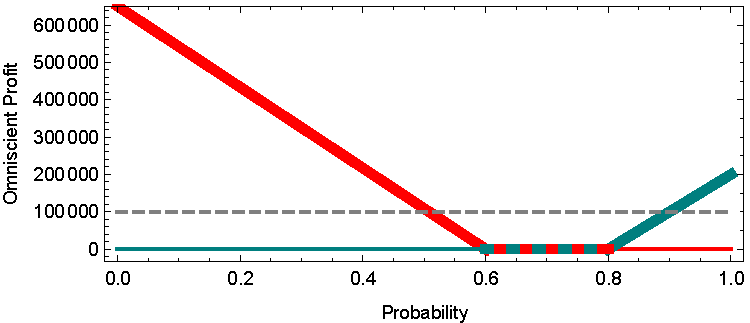
\includegraphics[width=\columnwidth]{god-profit.pdf}
\caption{
The thick line depicts the expected profit for a budget-unconstrained, omniscient bettor as a function of the true probability of Team A winning, $p$, in a market with current estimate $q=0.7$.
This is the maximum of the expected profit betting that Team A loses (in red) and betting that Team A wins (in green).
%The slightly steeper gradient on the left represents a (hypothetical) situation with more abundant trading opportunities betting on Team A losing.
The gray dashed line at \$100k omniscient profit implies a \$100k margin of error between its intercepts with the red and green lines.
This is the set of values of $p$ for which the omniscient bettor expects at most \$100k profit: $0.5\le p\le 0.9$ in this example.
The flat segment where red and green overlap ($0.6\le p\le 0.8$) indicates the set of probabilities consistent with a \$0 omniscient profit. 
The bid-ask spread is necessarily contained in this range.}
\label{fig:godprofit}
\vspace{-0.4cm}
\end{figure}

% In extreme-EMH world we could think of the dashed line as showing the range of probabilities that might become your own true objective probability if you spent up to \$100k gathering new information.

Note that many features of a market that we intuitively associate with increased accuracy will also be associated with narrow margins of error: high liquidity, no investment caps, and low fees.
All of these features increase the (expected) profit that an omniscient trader could extract from participating in the market, 
shrinking the space of true probabilities 
%$p$ 
that would result in a profit less than $\$x$.
%making it less likely that a given true probability $p$ would result in a profit less than $\$x$.

Consider (hypothetical) prediction markets for the professional and pickup football matches described in Section~\ref{sec:intro}. Due to the high information flow and level of interest in the professional match, we would expect a thick market with many opportunities for trade. The margin of error in this market will be narrow, because a trader with knowledge that the market was wrong could make a large profit. On the other hand, we would expect the market in the pickup game to be thinly trafficked. Even a trader who had precise knowledge of the capabilities of the teams would be able to make very little money. The margin of error in this market would be wide, reflecting a low confidence in the market estimate.

In the case of continuous double auction (CDA) markets,\footnote{In a CDA market, traders place bid offers to buy securities, and ask offers to sell, with the market matching all mutually beneficial offers. The gap between the highest bid and the lowest ask is known as the bid-ask spread.} the \$0 margin of error is always a superset of the bid-ask spread, since a trader whose belief lies within the spread has no buying or selling opportunities.
In the case of zero fees and no opportunity cost, the \$0 margin of error would coincide with the bid-ask spread exactly.

One can imagine prediction market estimates being reported in this way. 
For example, a
%news article or researcher 
data journalist
could report that the probability of Joe Biden being elected president is 65\%, with the \$1000 margin of error being between 57\% and 70\%. A market with a narrower margin of error at the $\$x$ level should be more trustworthy than a market with a wider margin of error.

This method can even extend to settings with multiple markets for the same event, or situations with very general betting structures that need not take the form of conventional prediction markets. When there are multiple markets (say, two different platforms each have a market for the same event), we can imagine an informed trader who is able to invest in all markets, profiting from each one. Since a trader can make higher expected profit from participating in two markets than just one, the margin of error that results from considering multiple markets will be no wider than the margin of error from considering a subset of those markets. Once again, this matches our intuition; additional information should not make us \emph{less} confident in our prediction. Similarly, in any betting situation, we can ask how much profit a bettor with infinite budget and precise knowledge of the underlying true probability $p$ could make in expectation, given the bets laid down by the other parties.

%Other question: If we say that the probability of some event is $p$, what does that mean? For God profit, shouldn't God know the 0/1 outcome? Is there a single point at which uncertainty is realized? Otherwise, if uncertainty is realized continuously between now and some definitive end date, does the fact that $p$ might change tomorrow really reflect that we are uncertain in our probability \emph{today}?

%%%%%%%%%%%%%%%%%%%%%%%%%%%%%%%%%%%%%%%%%%%%%%%%%%%%%%%%%%%%%%%%%%%%%%%%%%%%%%%%

%\vspace{-0.1cm}
\section{Confidence as Volatility}
\label{sec:options}

% \rupert{I don't really know what else to say here, but optically it's a bit weird having such a short section. Figure?}
% \dreev{idea: mention how this means explicitly having a meta market --- a market predicting the output of the first market. that could also be an excuse to cite pearl's anti-meta-probabilities paper~\cite{pearl1987} again. i'm keen to make sure the reader doesn't miss the fact that we haven't missed the fact that meta-probabilities are never needed.}

%Suppose that a coin will be flipped tomorrow. The coin to be flipped has not yet been decided, but will be one of two coins. One of the coins has a 0.7 probability of heads, and the other 0.5. The coin to be flipped will be chosen uniformly at random later today. 

Let us return to Game 2 from the introduction, in which a 50/50 random event will occur \emph{before} the football match in question, the outcome of which will inform us whether Team A has a 50\% or a 90\% chance of winning the match.

Can we say we're confident in today's estimate of 70\%?
By the measure we suggest in Section~\ref{sec:emh}, yes.
The information structure is public so we expect plenty of traders willing to bet if the implied odds deviate from 70\% in either direction.
But in another sense, no.
We're expecting new information, 24 hours before the game, that will render the 70\% estimate wrong in hindsight.
A layperson 
%being 
told that a probabilistic prediction has high confidence would be taken aback to see the prediction change drastically the following day.
We can capture that notion of confidence (or lack thereof) by measuring the expected \emph{volatility}.
A prediction with high expected volatility indicates, in our toy example, additional layers of uncertainty that will be resolved before the event itself resolves.

In financial markets, options and other derivatives reveal the distribution and variance of their underlying instruments. 
For example, a \emph{butterfly option} %is a contract that 
pays the absolute difference between the market price at time $t_1$ and the price at time $t_2$: $|p_{t_1}-p_{t_2}|$. 
Such contracts could be traded in a market secondary to any prediction, %market (or indeed, any prediction at all), 
allowing us to estimate the %expected
volatility of the primary prediction.

In other words, a %\emph{meta-market} 
\emph{second-order} market can predict volatility in the original market.
To be clear, second-order probabilities can always be collapsed into first-order probabilities~\cite{pearl1987}.
Nonetheless, the concept of second-order probabilities are well-defined and capture the expectation of new information that will change our probability estimate.
%As \citeauthor{pearl1987} discusses~\cite{pearl1987}, this would represent confidence as probabilities over %relevant information that is currently hidden.
%future %values of 
%probabilities.
For the example of Game 2, the price of the butterfly option would reveal that the current prediction, a $70\%$ chance of Team A winning, is expected to change by $\pm 20\%$ exactly when the COVID-19 test occurs.
This would reflect a lack of confidence in the prediction, at least relative to that point in the future.

We believe that this ``volatility'' notion of confidence is complementary to the ``$\$x$ margin of error'' notion of confidence.
One can imagine scenarios, such as the Game 2 example, where the $\$x$ margin of error is very small while the volatility is large.
The converse appears possible, but less likely: a high $\$x$ margin of error implies high uncertainty about the current prediction, which suggests volatility of the price in the future.
In any case, both measures together may give a clearer picture of the market's confidence.

%While we can be confident in that probability, we also know that more information is going to arise that will render our current probability estimate of 0.6 inaccurate (in hindsight). Here, the additional stage of uncertainty is reflected in the increased volatility of the prediction between now and the outcome being realized.

%For concreteness, suppose that a binary event will be realized at time $t$ in the future. Further, let us assume that by time $t-1$ the true probability (or at least a best estimate of the probability, incorporating all relevant and knowable information) $p$ of the event will be known. One measure of our confidence in our current estimate of the probability $q$ is the expected absolute difference between $p$ and $q$. While $q$ is our current best guess as to the probability, a high expected absolute difference indicates that we do not believe $q$ accurately reflects the uncertainty inherent in the event, while a low expected absolute difference indicates that we do.

%While the expected absolute difference between $p$ and $q$ could be estimated in a variety of ways, one way to do so is to employ a market, allowing traders to buy and sell contracts that realize a value $|p-q|$ after time $t$. The value of these contracts at any point in time is equal to the expected volatility of the prediction between now and time $t-1$.

% One may reasonably question whether expected volatility reflects uncertainty in the current prediction. After all, in our two-stage coin flip example above, the 0.5 probability perfectly and completely captured the uncertainty present in the process. However, it was not a good estimate of the randomness inherent only in the second stage, the flipping of the chosen coin, precisely because it incorporated some additional randomness that was resolved before the flip. The expected volatility is a way to quantify how much of the relevant information has already been observed relative to how much is yet to be observed. It seems to us \rupert{Or at least, to me} that if a large amount of information about a random event is yet to be received, that implies uncertainty in the current prediction.

%%%%%%%%%%%%%%%%%%%%%%%%%%%%%%%%%%%%%%%%%%%%%%%%%%%%%%%%%%%%%%%%%%%%%%%%%%%%%%%%

%\vspace{-0.1cm}
\section{Discussion and Challenges}
\label{sec:discussion}

\subsection{Evaluating a Measure of Confidence}
\label{sec:evaluation}

So far, we have avoided defining confidence formally, instead appealing to intuition about the nature of a confident forecast. However, before these notions can be used, they need to be validated empirically and/or theoretically, which necessitates a definition. 
For the purpose of illustration, let us define a probabilistic prediction $q$ to be \emph{accurate} if it is close to the true probability $p$. 
We can then define a confident forecast as one that we believe to be accurate, that is, to properly reflect the inherent randomness.

If we accept this definition, we would hope that a confident prediction would, on average, be more accurate than a less confident one. 
Measuring accuracy is challenging in itself, since we never observe true probabilities $p$, but instead only the event outcomes. While it is possible to score predictions in such a way that more accurate predictions receive higher scores in expectation than less accurate ones~\cite{brier1950verification,gneiting2007strictly}, it is impossible to know if a single prediction is accurate or not.

%Comparing two predictions may be hard, but
%Comparing two forecasters is relatively easy.
If two forecasters each predict the same set of events and each forecast is scored, the more accurate forecaster will achieve the higher score
%a higher score than the less accurate forecaster 
over time. 
One may hope that this technique would allow us to validate a measure of confidence, in the sense that high-confidence forecasts should achieve a higher score on average than low-confidence forecasts if confidence is indeed reflecting accuracy.

Unfortunately, to do this would require a set of high-confidence predictions and low-confidence predictions \emph{for the same set of events}. Otherwise, an accurate prediction of $q=p=0.5$ may receive a lower score, even in expectation, than an erroneous prediction $q=0.8$ of a different event with $p=0.9$. Due to the intertwined nature of real-world markets, finding such a pair of markets for any event is a difficult, perhaps impossible, proposition. To pursue this direction, markets may need to be created in laboratory conditions, or a more clever evaluation method designed.

Additionally, we may want a way to interpret market confidence in an absolute sense, not relative to another market, in the same way that polling margin of errors have a precise interpretation as confidence intervals. This would seem to be a very challenging question to resolve empirically, since we never observe the underlying probabilities. Perhaps it is a question better suited to a theoretical modeling approach, in which (hypothetical) traders observe some information, trade is simulated, and the features of the corresponding market observed.

%It is well known that some (human, machine, or combination) forecasters are more accurate than others. This can be easily established by having a group of forecasters make predictions on a series of events, and then to score those predictions according to a proper scoring rule such as the quadratic or logarithmic scoring rule~\cite{the canonical hanson paper?}. It is easy to understand what it would mean for such an accuracy measure to generalize. If all forecasters make a prediction on some new events, do high-accuracy forecasters achieve higher scores, on average, than low-accuracy forecasters?

%On the other hand, we propose measuring accuracy on a market-by-market basis. Each market is different, with its own unique features,\footnote{Fee structures may be the same across many markets on a single platform, but the trading patterns in each market will be unique.} so we are unable to have the same market make multiple predictions in order to get a true picture of whether it is an ``accurate'' market or not. However, we would still like to evaluate how ``confidence,'' as measured by some metric, is reflected in the relationship between market predictions and outcomes.

\subsection{Model variants}

Much of our discussion so far has been predicated on the idea that every event has some inherent and unknowable, yet quantifiable and well-defined, uncertainty occurring at a precise moment in time. Alternative models are of course possible, and may affect how we define and think about uncertainty. This gets much more complicated as the speed of information shifts: our examples take place before a football game, when new information is relatively slow, versus during a football game when new information comes rapidly. While these periods are relatively well defined for sports, they are more ambiguous for politics: did the 2024 presidential election start before or after the 2020 presidential election ended? Announcements and debates happen periodically, shaking probabilities. 
During times of particularly intense new information (like during a football game or political debate), uncertainty can shift rapidly, and market volume generally increases dramatically. Our key indicators of bidding and price tend to behave very differently during these periods than in times of low information flow, possibly shifting their relationship to confidence.
%During times of particularly intense new information (like during a football game or political debate), uncertainty can shift rapidly, and in markets, due to excitement and mechanics of betting, volume generally increases dramatically, and our key indicators of bidding and price tend to behave very differently than in times of low information flow, possibly shifting their relationship to confidence.
%\rupert{This subsection used to be titled ``Knowable and Unknowable Uncertainty'' but I didn't really get there explicitly. I'm not sure that the omniscient profit notion really relies on unknowable uncertainty. We could always imagine a trader who simply believes that the market is wrong and ask how much they would make in (subjective) expectation. Am I missing something?} 

% This is messing up where the footnotes are placed; commented out for now:
%\balance % balance columns on last page; must occur last page's in left column, weirdly
% PS: never mind, apparently now it's doing the balancing just fine without this!

%\subsection{Manipulation}
%
% In almost all situations, predictions are used to shape actions. Political candidates focus their attention on close races, predicted health outcomes inform treatments, economic forecasts are used to set monetary policy. Knowing the confidence in a prediction naturally informs information acquisition: if a prediction is confident (insofar as it would change my action) then I can safely move forward without acquiring more information, otherwise I should.

\subsection{Value of Information}

The notions of confidence in Sections~\ref{sec:emh} and~\ref{sec:options} can both be interpreted in terms of the value of information acquisition. In Section~\ref{sec:emh}, an equivalent interpretation of the $\$x$ margin of error is that it contains all the predictions that could result if a forecaster spent $\$x$ acquiring new information (otherwise, a forecaster could make greater than $\$x$ profit from the market by spending only $\$x$ on information acquisition, violating the efficient market hypothesis\footnote{In reality, we don't expect markets to be so efficient that this holds exactly.}). In Section~\ref{sec:options}, the expected market volatility expresses how much we expect the prediction to change as new information comes to light. High expected volatility says that the new information will be highly valuable compared to old information.
%, while low expected volatility says the opposite. \dreev{quibble: low expected volatility means we don't expect new information to come to light; it may be very valuable if it did!}
Further exploring the relationship between value of information and market confidence may be fruitful.
%\rupert{Dan, I loved the way you phrased this in your email. I've tried to translate that elegance here, but feel free to do a better job.}


\subsection{Communicating probabilistic uncertainty}

Regardless of the precise definition of confidence in a prediction, we're interested in how to convey it to a lay audience.
%it is interesting to consider how the notion can be communicated to a lay audience. 
For example, one way to conceptualize a 20\% probability is to imagine 20 red balls and 80 blue balls. 
The probability of the event occurring is the same as a randomly chosen ball being red. 
Could we use the same analogy to communicate an imprecise probability, where the number of red balls 
%is unknown but 
may be anywhere between 16 and 24? 
What about if some numbers of red balls are more likely than others? 
Of course, the exercise could be repeated for a host of probability explanation and visualization tools.

\subsection{Deriving a single probability from a market}

Our discussion has been phrased in terms of second-order uncertainty: how confident can we be that a probabilistic prediction accurately reflects the inherent underlying randomness. However, even in the presence of second-order uncertainty, a Bayesian agent must be able to represent their belief by a single probability~\cite{pearl1987}. 
How best to derive a probability from a real-world prediction market remains an open problem.
In a hypothetical high-liquidity LMSR with no fees and no opportunity cost for tying up funds, the market price should be our best estimate of the underlying probability.
For a real-world continuous double auction market with a bid-ask spread, how do we infer a probability from what the market is telling us?
Plausibly the midpoint of the bid-ask spread is the best we can do but that's an empirical question worth answering.
Other hypotheses include (a) the edge of the bid-ask spread closest to or furthest from 50\%, due to known distortion effects in markets at extreme probabilities, (b) something outside the bid-ask spread that accounts for fees and opportunity cost, (c) a more elaborate, perhaps machine-learned, function of the order book.

\begin{comment}
If we get a list of bid-ask spreads along with final outcomes, we can ask ``for what convex combination (or fancier function) of bid and ask do we get the highest average Brier score, or best calibration?''
For example, maybe the low end of the range does best, or the bid/ask boundary furthest away from 0.5, or maybe everything in [bid, ask] is equally good.
%We'd want to split the data into training and test sets, etc.
\end{comment}

%\rupert{Outside interest, manipulation, observing order book, true probability/inherent randomness}

The right way to derive a single probability is, in principal, solved by Bayesian theory: (1) start with a joint prior over the events and the markets, (2) treat all attributes of the markets as evidence, and (3) compute the posterior. This is called the \emph{supra-Bayesian} approach to aggregating probabilities~\cite{winkler1968, morris1974, morris1977,Lindley85,Lindley88}. Although this approach is correct in theory, it sidesteps all the hard practical problems: how does the agent generate and represent a joint prior encoding every detail about how evidence from markets correlates with events, and compute the posterior tractably?

%%%%%%%%%%%%%%%%%%%%%%%%%%%%%%%%%%%%%%%%%%%%%%%%%%%%%%%%%%%%%%%%%%%%%%%%%%%%%%%%
%%%%%%%%%%%%%%%%%%%%%%% ACKNOWLEDGMENTS AND BIBLIOGRAPHY %%%%%%%%%%%%%%%%%%%%%%%
%%%%%%%%%%%%%%%%%%%%%%%%%%%%%%%%%%%%%%%%%%%%%%%%%%%%%%%%%%%%%%%%%%%%%%%%%%%%%%%%

% \begin{acks}
% We should thank (at least) Jenn here.
% Bethany Soule read a draft and pointed out all sorts of awkward things that I'm working on improving.
% \end{acks}

\bibliographystyle{ACM-Reference-Format} 
\bibliography{oddable}

\end{document}

%%%%%%%%%%%%%%%%%%%%%%%%%%%%%%%%%%%%%%%%%%%%%%%%%%%%%%%%%%%%%%%%%%%%%%%%%%%%%%%%
%%%%%%%%%%%%%%%%%%%%%%%%%%%%%%%% SCRATCH NOTES %%%%%%%%%%%%%%%%%%%%%%%%%%%%%%%%%
%%%%%%%%%%%%%%%%%%%%%%%%%%%%%%%%%%%%%%%%%%%%%%%%%%%%%%%%%%%%%%%%%%%%%%%%%%%%%%%%

more citation ideas:

1. Taleb: "Election Predictions as Martingales: An Arbitrage Approach".  
<https://arxiv.org/pdf/1703.06351.pdf>
2. "Arbitrage in Political Prediction Markets".  
<http://www.bjll.org/index.php/jpm/article/view/1796>
3. Gelman et al: "Information, incentives, and goals in election forecasts".  
<http://www.stat.columbia.edu/~gelman/research/published/jdm200907b.pdf>
4. Taleb vs Silver primer:  
<https://towardsdatascience.com/why-you-should-care-about-the-nate-silver-vs-nassim-taleb-twitter-war-a581dce1f5fc>
5. Schmitz and Rothschild: "Understanding market functionality and trading success".  
<https://journals.plos.org/plosone/article?id=10.1371/journal.pone.0219606>
6. Crane and Vinson: Preregistered comparison of polls vs markets.  
<https://researchers.one/articles/Models-vs-Markets-Forecasting-the-2020-US-election/97212967bc124e2bf3af31a5>


dpenn: 

2. The game theory aspects: as a single agent, my confidence in a probability doesn't matter. 
As an agent playing in a game with other agents, my confidence matters, with the extreme case being the no-trade theorems.

3. The empirical machine learning approach: 
try to learn a function from all the attributes of a market price, including god profit, to the expected quadratic score of that price.


dreev thinking out loud:

1. Probability is not a fact about nature; it is a fact about you. It measures how complete or incomplete your knowledge is. You can think of it in terms of rational decision-making, as a measure of what bets you should make. That's ``bet'' in a very general sense: the probability of rain measures how you'll trade off the hassle of carrying an umbrella against the unpleasantness of getting wet.

2. We can derive a probability from a market in an unambiguous way and that probability will then be your own true subjective probability, assuming you have no source of information other than the market.

3. Prediction confidence is something orthogonal. Your probability is your probability but your confidence in your probability can refer to a couple things.
First, you may expect your probability to change as new information comes to light. This is known in finance as volatility and --- if your probability is determined by the price of a security in a market --- can be measured by a financial derivative of that security.
Second, you may expect that your probability \emph{could} change if you spent resources to acquire more information.

4. We can use the God profit / dollar interval idea to compute a range of probabilities that your true probability might move to if you were to spend up to \$x gathering new information.

5. That kind of assumes EMH but there's a similar thing we can say without EMH. Namely, if you disagree with the market within a given range, you stand to profit at most \$x.

Extreme EMH: The market is in a pristinely arbitrage-free state where all information that's profitable to incorporate has been incorporated and the omniscient profit graph is telling you how much you'd have to spend acquiring new information to move the probability within a given range.

more thinking out loud:
maybe we should mention that plain old liquidity counts as a measure of market confidence: tightness of bid-ask spread and being able to put in a lot of money without moving the market price. i guess that's what god profit is quantifying...

All the combinations of our two confidence measures. Sanity check:

1. high volatility, tight dollar intervals = big new info is coming and everyone knows it (Game 2)
2. high volatility, wide dollar intervals = [this is the one that seems unlikely to arise in practice?]
3. low volatility, tight dollar intervals = big sports game with no new info coming (Game 1)
4. low volatility, wide dollar intervals = pickup game, no one knows but info is gatherable (Game 3)